
\begin{figure}[h!]
\centering
\begin{subfigure}[b]{0.9\textwidth}
\centering
\hspace{-0.7cm}
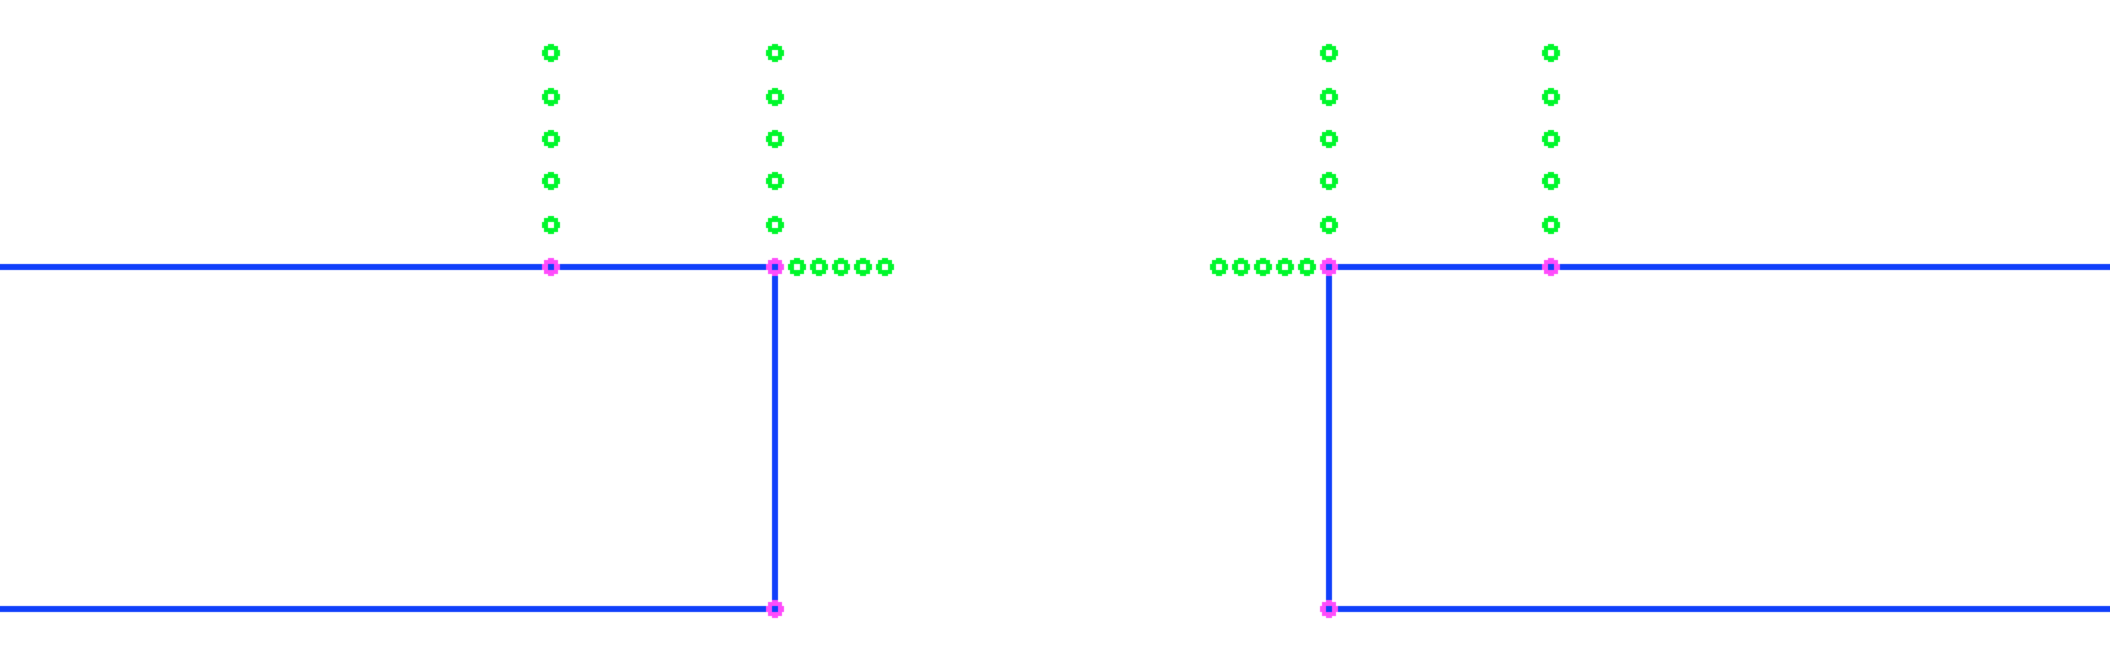
\includegraphics[width=8cm, height=3cm]{normals_points}
\end{subfigure}
\begin{subfigure}[b]{0.4\textwidth}
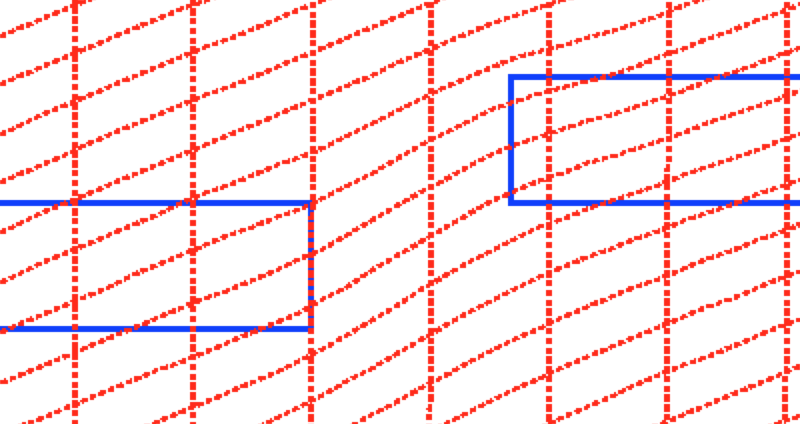
\includegraphics[width=6cm, height=3cm]{TPS_withoutnormals}
\caption{}
\end{subfigure}
\hspace{0.02\textwidth}
\begin{subfigure}[b]{0.4\textwidth}
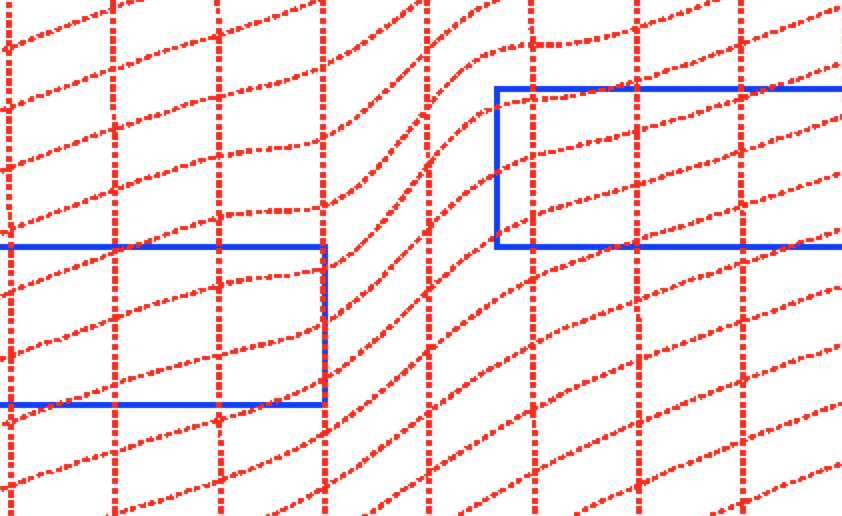
\includegraphics[width=6cm, height=3cm]{TPS_withnormals}
\caption{}
\end{subfigure}
\caption{The demonstration scene (top image) has two suturing pads aligned in the same horizontal plane. In the test scene (bottom two images) the right pad is shifted upwards. (a) Warp found by TPS using six pairs of correspondence points between the scenes, indicated by the magenta points. (b) Warp found by TPS after adding in correspondence points along the relevant normals, indicated by the green points. The second warp is more likely to effectively generalize trajectories as it better captures the structure of the scene.}
\label{fig:normals}
\end{figure}
When using thin plate splines to generalize manipulation trajectories fails, it is often because the warping function that is found does not preserve important geometric properties of the scene. A common failure mode arises because the warping function fails to preserve surface normals. For example, consider the manipulation task of suturing two pads of tissue. One important aspect of this task is the suturing needle's angle of entry into the pads. However, in situations where the pads are offset vertically relative to the demonstration, the warping function that minimizes error on the correspondence points rarely captures this. Figure~\ref{fig:normals} shows a two dimensional illustration of this problem. One approach for making this trajectory transfer more robust is to include correspondences on surface normals. As an initial investigation, we model this type of constraint by introducing new point correspondences to model the surface normals, shown in Figure~\ref{fig:normals}. We found through experimenting with this approach that it leads to interpolating splines that generalize demonstrations more effectively. 

However, we would like to find a more principled way to incorporate these surface normal correspondences into the thin plate spline optimization. Formally, we want to find a mapping between $m$ normals \ns{l}, $l=1,...,m$, at respective positions \xes{l} in the source scene, and the respective normals \nt{l} in the target scene. A natural way to map a surface normal (or any vector) through a function like this is to make use of the tangent space. In differential geometry, this is the idea of a pushforward operator~\cite{ralph1978foundations}. In our setting, mapping a normal $\ns{l}$ through a thin plate spline function $f$ at a point $\xes{l}$ corresponds to multiplying by $J_f(\xes{l})$, the Jacobian of $f$ at $\xes{l}$: $$J_f(\xes{l}) \cdot \ns{l}.$$  

Thus, correspondences between normals in two scenes result in constraints on the Jacobian of $f$, while correspondences between points result in constraints on the value of $f$. Incorporating this into the thin plate spline objective, we get the following problem:
\begin{equation}
\begin{align}
 &\underset{f}{\text{minimize\ \ \ }} & ||f||_{tps}^2 \\
 &\text{subject to\ \ \ }
 & \xt{i} = f(\xs{i}) \\
 && \nt{l}= J_f(\xes{l}) \cdot \ns{l}\\
\end{align}
.
\label{eq:tps_normals}
\end{equation}

Alternatively, we can trade off between the error on the correspondences and the smoothness of our curve with the following objective
\begin{equation}
f = \underset{f}{\text{argmin}} \sum_{i=1}^k ||\xt{i} - f(\xs{i})||_2^2 + \sum_{l=1}^m ||\nt{l} - J_f(\xes{l}) \cdot \ns{l}||_2^2 + \lambda ||f||_{tps}^2.
\label{eq:tps_normals_reg}
\end{equation}

Bookstein and Green show an approximation method to solve Equation~\ref{eq:tps_normals}, in which $f$ can be expressed as a weighted sum of slope functions and the landmark-only TPS basis functions $\mathbf{b}$~\cite{BooksteinGreen}. The slope functions $U_{\mathbf{t}$ are the derivative of $U$ in the direction $\mathbf{t}$. In 2D, we have
\begin{equation}
\begin{align*}
U_{\mathbf{t_i}}(\mathbf{x}) &= \mathbf{t_i} \cdot \nabla U(\mathbf{x}) \\
&= (2 \ln ||\mathbf{x}|| + 1)(\mathbf{x} \cdot \mathbf{t_i}) .
\end{align*}
\end{equation}

Then $f$ can be written as
\begin{equation}
f(\mathbf{x}) =
E^\top
\begin{bmatrix} 
  \mathbf{b}^\top &
  -U_{\ns{1}}(\mathbf{x}-\xes{1}) &
  -U_{\ns{2}}(\mathbf{x}-\xes{2}) &
  \cdots &
  -U_{\ns{m}}(\mathbf{x}-\xes{m})
\end{bmatrix}^\top
\end{equation}
where $E$ is the weight matrix that minimizes the objective in Equation~\ref{eq:tps_normals}. Recall that $\mathbf{b}$ has the landmark-only TPS basis fuctions
\begin{equation}
\mathbf{b} =
\begin{bmatrix} 
  U(\mathbf{x} - \xs{1}) & U(\mathbf{x} - \xs{2}) & \cdots & U(\mathbf{x} - \xs{k}) & \mathbf{x}^\top & 1
\end{bmatrix}^\top .
\end{equation}

